\section{Regularization tuning}

First of I tried to tune the parameters of the logistic regressor. As I see it,
the only parameter worth touching --- at least for this exercise --- is the C,
or regularization parameter. However, changing it didn't have much of an
effect, and the scikit-learn default, 1, seems to perform the best.
Graph~\ref{fig:reg_tuning} depicts the effects of changing the parameter.

\begin{figure}[H]
  \centering
  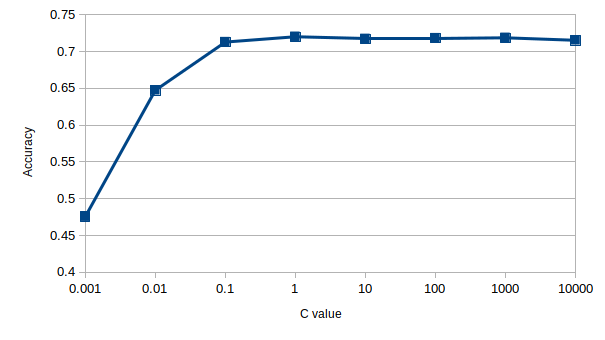
\includegraphics[width=0.8\linewidth]{reg_tuning}
  \caption{Effect of the regularization parameter on classifier accuracy}\label{fig:reg_tuning}
\end{figure}



\section{Tuning the n-grams parameter on word vectorization}

Changing the n-gram range parameter on the word count vectorization had a
bigger effect. The n-gram range option in this case means how many words are
considered as a feature. The optimum value seemed to be a range of \(1-2\).
Table~\ref{tab:ngram} has some different results.

\begin{table}[H]
  \centering
  \caption{Some n-gram range values used in word count vectorization and the
  resulting accuracy}\label{tab:ngram}
  \begin{tabular}{c c}
    \toprule
    (1, 2)  &  \num{0.739563106796116} \\
    (1, 3)  &  \num{0.735194174757281} \\
    (1, 4)  &  \num{0.722087378640776} \\
    (2, 2)  &  \num{0.711407766990291} \\
    (2, 3)  &  \num{0.697572815533980} \\
    (2, 4)  &  \num{0.683009708737864} \\
    (3, 3)  &  \num{0.616990291262135} \\
    (3, 4)  &  \num{0.590048543689320} \\
    (4, 4)  &  \num{0.495631067961165} \\
    \bottomrule
  \end{tabular}
\end{table}



\section{Trying out tf-idf}
Perhaps somewhat surprisingly (at least to me), the results using term
frequency were significantly worse than just using the word counts. The best
score (obtained by (1,1) ngram range) was just \num{0.6973300970873786}, which
is worse than even the baseline.



\section{Using the unlabeled data}

The best results were gotten by adding some unlabeled data into the mix. The
best accuracy on the development set is \num{0.7487864077669902}, and that was
achieved when adding 19,000 unlabeled samples to the training set.

The method for using the unlabeled data was the same as the first method
described in the assignment description. To reiterate, we train the classifier
on the labeled training set. Then we predict some labels for a part of the
unlabeled set, I used a batch size of 100. Then we add that data into the
``labeled'' training set and repeat the process. In my implementation we just
go through all the unlabeled data in this manner. As we can see from the
graph~\ref{fig:unlabeled}, this works fairly well as the performance increases
when add most of the unlabeled samples.


\begin{figure}[H]
  \centering
  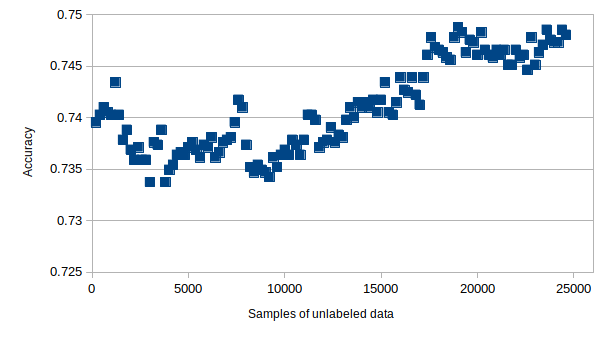
\includegraphics[width=0.8\linewidth]{unlabeled}
  \caption{A XY-plot of the effect of adding unlabeled data samples to the
  training}\label{fig:unlabeled}
\end{figure}






















